\subsection{1-reducibility of ring $R_5$}

\begin{frame}
    \frametitle{1-reducibility of ring $R_5$}

    \begin{theorem}<1->
        The ring $R_5$ is 1-reducible
    \end{theorem}

    \uncover<2->{
        \textit{Proof.} We will show that there is a common ring coloring for any $M+S$ and $\core + S'$.

        Let the ring colorings of the two graphs again be given by
        \begin{equation}
            \I = \Phi(M+S) \quad \text{and} \quad \II = \Phi(\core+S').
        \end{equation}

        We can choose to reduce with any $S$ and $S'$ on $\leq 1$ extra vertices. Each choice gives us guaranteed colorings for I and II.
    }
\end{frame}

\begin{frame}
    \frametitle{1-reducibility of ring $R_5$}
    First we examine the guaranteed colorings without using a reducer.

    \begin{figure}[!ht] 
        \centering
        \begin{tikzpicture}[mid arrow/.style={
            postaction={ decorate, decoration={ markings, mark=at position 0.6 with { \arrow[black]{>>} } } } }]
            \draw[fill=white] (-0.5, 0) ellipse (2cm and 1.5cm);
            \node (m) at (-1.7, 0) {$M$};
            \node at (-0.8, 0.8) {$R_5$};
    
            \node[circle, fill, scale=0.015cm] (l1) at (0, 1) { };
            \node[circle, fill, scale=0.015cm] (l2) at (0.9, 0.30) { };
            \node[circle, fill, scale=0.015cm] (l3) at (0.6, -0.77) {};
            \node[circle, fill, scale=0.015cm] (l4) at (-0.6, -0.77) {};
            \node[circle, fill, scale=0.015cm] (l5) at (-0.9, 0.30) {};
            \draw[mid arrow] (l1) -- (l2);
            \draw (l2) -- (l3) -- (l4) -- (l5) -- (l1);
        \end{tikzpicture}
        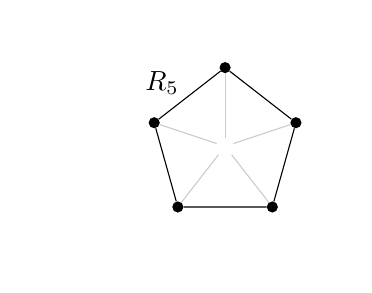
\begin{tikzpicture}[mid arrow/.style={
            postaction={ decorate, decoration={ markings, mark=at position 0.6 with { \arrow[black]{>>} } } } }]
            \draw[opacity=0] (-0.5, 0) ellipse (2cm and 1.5cm);
            \node at (-0.8, 0.8) {$R_5$};
            \node[inner sep=1mm] (c) at (0, 0) {$\core$};
            \node[circle, fill, scale=0.015cm] (l1) at (0, 1) { };
            \node[circle, fill, scale=0.015cm] (l2) at (0.9, 0.30) { };
            \node[circle, fill, scale=0.015cm] (l3) at (0.6, -0.77) {};
            \node[circle, fill, scale=0.015cm] (l4) at (-0.6, -0.77) {};
            \node[circle, fill, scale=0.015cm] (l5) at (-0.9, 0.30) {};
    
            \draw[opacity=0.2] (c) -- (l1);
            \draw[opacity=0.2] (c) -- (l2);
            \draw[opacity=0.2] (c) -- (l3);
            \draw[opacity=0.2] (c) -- (l4);
            \draw[opacity=0.2] (c) -- (l5);
            \draw (l1) -- (l2) -- (l3) -- (l4) -- (l5) -- (l1);
        \end{tikzpicture}
        \caption{The reductions $M+R_5$ and $\core+R_5$.}
        \label{fig:ring5k0}
    \end{figure}

    These plain rings $R_5$ in each graph may be further reduced by contracting two opposing vertices.
    
\end{frame}

\begin{frame}
    \frametitle{1-reducibility of ring $R_5$}
    
    We can contract two opposing vertices of $R_5$ in 5 different ways. Each choice guarantees a coloring where two vertices are colored the same.

    \uncover<2->{
    \begin{equation}
        \Phi^\star = \{ a{*}{*}a{*}, \quad {*}a{*}{*}a, \quad a{*}a{*}{*}, \quad {*}a{*}a{*}, \quad {*}{*}a{*}a{*} \}.
    \end{equation}
    }

    \uncover<3->{
        The ${*}$-colors are still unknown, but we are guaranteed that the colorings are possible, therefore $\Phi^\star \subset \I,\II$.
    }
\end{frame}

\begin{frame}
    \frametitle{1-reducibility of ring $R_5$}

    Next, we examine the guaranteed colorings with a reducer that has 1 extra vertex.

    \uncover<2->{\begin{figure}[!ht]
    \centering
    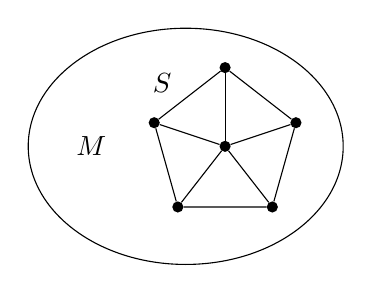
\begin{tikzpicture}[mid arrow/.style={
        postaction={ decorate, decoration={ markings, mark=at position 0.6 with { \arrow[black]{>>} } } } }]
        \draw[fill=white] (-0.5, 0) ellipse (2cm and 1.5cm);
        \node (m) at (-1.7, 0) {$M$};
        \node at (-0.8, 0.8) {$S$};

        \node[circle, fill, scale=0.015cm] (l1) at (0, 1) { };
        \node[circle, fill, scale=0.015cm] (l2) at (0.9, 0.30) { };
        \node[circle, fill, scale=0.015cm] (l3) at (0.6, -0.77) {};
        \node[circle, fill, scale=0.015cm] (l4) at (-0.6, -0.77) {};
        \node[circle, fill, scale=0.015cm] (l5) at (-0.9, 0.30) {};
        \node[circle, fill, scale=0.015cm] (e) at (0, 0) { };

        \draw (e) -- (l1);
        \draw (e) -- (l2);
        \draw (e) -- (l3);
        \draw (e) -- (l4);
        \draw (e) -- (l5);
        \draw (l1) -- (l2);
        \draw (l2) -- (l3) -- (l4) -- (l5) -- (l1);
    \end{tikzpicture}
    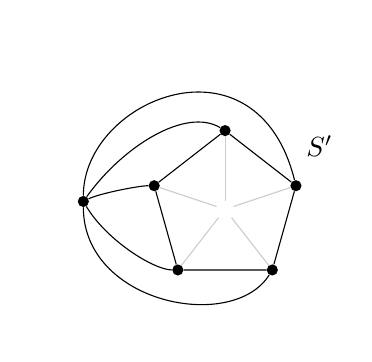
\begin{tikzpicture}[mid arrow/.style={
        postaction={ decorate, decoration={ markings, mark=at position 0.6 with { \arrow[black]{>>} } } } }]
        \draw[opacity=0] (-0.5, 0) ellipse (2cm and 1.5cm);
        \node[fill=white] at (1.2, 0.8) {$S'$};
        \node[inner sep=1mm] (c) at (0, 0) {$\core$};
        \node[circle, fill, scale=0.015cm] (l1) at (0, 1) { };
        \node[circle, fill, scale=0.015cm] (l2) at (0.9, 0.30) { };
        \node[circle, fill, scale=0.015cm] (l3) at (0.6, -0.77) {};
        \node[circle, fill, scale=0.015cm] (l4) at (-0.6, -0.77) {};
        \node[circle, fill, scale=0.015cm] (l5) at (-0.9, 0.30) {};
        \node[circle, fill, scale=0.015cm] (e) at (-1.8, 0.1) { };

        \draw (e) .. controls +(0.2, 0.1) and + (-0.2, 0.0) .. (l5);
        \draw (e) .. controls +(0.3, -0.5) and +(-0.3,0) .. (l4);
        \draw (e) .. controls +(0.0,-1.3) and +(-0.5,-0.8) .. (l3);
        \draw (e) .. controls +(0.0,+1.3) and +(-0.5,+2) .. (l2);
        \draw (e) .. controls +(0.5,0.7) and +(-0.5, 0.3) .. (l1);

        \draw[opacity=0.2] (c) -- (l1);
        \draw[opacity=0.2] (c) -- (l2);
        \draw[opacity=0.2] (c) -- (l3);
        \draw[opacity=0.2] (c) -- (l4);
        \draw[opacity=0.2] (c) -- (l5);
        \draw (l1) -- (l2) -- (l3) -- (l4) -- (l5) -- (l1);
    \end{tikzpicture}
    \caption{The reductions $M+S$ and $\core+S'$.}
\end{figure}}

    \uncover<3->{
        These reducers guarantee \textbf{one} 3-coloring of the ring.
    }
\end{frame}

\begin{frame}
    \frametitle{1-reducibility of ring $R_5$}

    These reducers guarantee \textbf{one} 3-coloring of the ring $R_5$.

    \uncover<2->{
    \begin{equation}
        \Phi^S = \{ 
            \underline{c}abab\;\;\textbf{or}\;\; 
            a\underline{c}bab\;\;\textbf{or}\;\;
            ab\underline{c}ab\;\;\textbf{or}\;\;
            aba\underline{c}b\;\;\textbf{or}\;\;
            abab\underline{c} \}.
    \end{equation}
    }

    \uncover<3->{
        In total, we are guaranteed of two sets of colorings for $\I$ and $\II$.

        \begin{equation*}
            \Phi^\star, \Phi^S \; \subset \I,\II.
        \end{equation*}

        Next, we show that these guaranteed colorings are sufficient to find a common coloring in $\I$ and $\II$.
    }
\end{frame}

\begin{frame}
    \frametitle{1-reducibility of ring $R_5$}
    The 3-colorings are important because of two key properties that they have.

    \begin{definition}<2->
        The uniquely-colored vertex of a 3-coloring of $R_5$ is called the \emph{marked vertex}, indicated by an underline such as in $\underline{c}abab$.
    \end{definition}
    
    \begin{definition}<3->
        Two 3-colorings of $R_5$ are called \emph{adjacent} if they have adjacent marked vertices, such as in $\underline{c}abab$ and $a\underline{c}bab$.
    \end{definition}
\end{frame}

\begin{frame}
    \frametitle{1-reducibility of ring $R_5$}
    Both sets $\I$ and $\II$ are guaranteed to have one 3-coloring from $\Phi^S$. There are three cases that can occur.

    \vspace{1cm}
    \begin{enumerate}
        \uncover<2->{\item $\I$ and $\II$ have an adjacent coloring ($\underline{c}abab$ and $a\underline{c}bab$).}
        \uncover<3->{\item $\I$ and $\II$ have a non-adjacent coloring ($\underline{c}abab$ and $ab\underline{c}ab$).}
        \uncover<4->{
        \item $\I$ and $\II$ have a coloring with the same marked vertex ($\underline{c}abab$ and $\underline{d}cbcb$). These are already equal, so we are done.
        }
    \end{enumerate}
\end{frame}

\begin{frame}
    \frametitle{1-reducibility of ring $R_5$}

    \begin{enumerate}
        {\item $\I$ and $\II$ have an adjacent coloring ($\underline{c}abab$ and $a\underline{c}bab$).}
        {\item $\I$ and $\II$ have a non-adjacent coloring ($\underline{c}abab$ and $ab\underline{c}ab$).}
    \end{enumerate}

    \vspace{0.5cm}
    We have two lemmas to deal with these cases. Together they guarantee a common coloring in $\I$ and $\II$.

    \begin{equation*}
        \begin{aligned}
        \circled{2} \implies\; &\circled{1}\quad \text{or} \quad \text{common coloring} \quad\quad \text{(Lemma 1)} \\
        &\downarrow \\
        &\circled{1} \implies\;\text{common coloring}\quad\quad \text{(Lemma 2)}
        \end{aligned}
    \end{equation*}
    
\end{frame}

\begin{frame}
    \frametitle{1-reducibility of ring $R_5$}
    \begin{block}{Lemma 1}
        If $\I$ and $\II$ have a non-adjacent coloring, then they either have an adjacent coloring or a common coloring.
    \end{block}
    \uncover<2->{
        \textit{Proof.} Assume we have two non-adjacent colorings $\I(\underline{c}abab)$ and $\II(ab\underline{c}ab)$.
        Suppose that $v_3 \stackrel{bc}{\frown} v_5$ in $\II(ab\underline{c}ab)$. This leads to
    }
    \uncover<3->{
        \begin{equation}
            \begin{aligned}
                \II(ab\underline{c}ab) &=\scheme{a,b,c,a,b}{35b} \compat \II(abcdb), \\
                \II(ab\underline{c}ab) &= \scheme{a,b,c,a,b}{35b-} \compat \II(a\underline{c}bab).
            \end{aligned}
        \end{equation}
    }

    The second case results in a coloring adjacent to $\I(\underline{c}abab)$ as desired.
\end{frame}

\begin{frame}
    \frametitle{1-reducibility of ring $R_5$}
    The first case results in $\II(abcdb)$.
    \uncover<2->{
        Consider the coloring $\I({*}b{*}{*}b)$.
    }

    \uncover<3->{
        The two adjacent ${*}$-colors must be different from each other and $b$, therefore we may assume that we have $\I({*}bcdb)$. The last ${*}$-color reveals 3 possibilities.
    }
    \vspace{0.5cm}
    \uncover<4->{
        \begin{equation}
            \begin{matrix*}[l]
                \I(abcdb) \quad\quad =&\II(abcdb) \; \text{from case 1,}  \\
                \I(cbc\underline{d}b) \;\; \text{adjacent to}&\II(ab\underline{c}ab), \;  \\
                \I(db\underline{c}db) \quad\quad =&\II(ab\underline{c}ab).
            \end{matrix*}
        \end{equation}
    }
    \uncover<5->{
        Therefore we obtain either a common coloring or an adjacent coloring $\qedsymbol$.
    }
\end{frame}

\begin{frame}
    \frametitle{1-reducibility of ring $R_5$}
    \begin{block}{Lemma 2}
        If I and II have an adjacent coloring, then they have a common coloring.
    \end{block}
    \uncover<2->{
        \textit{Proof.} Assume we have two adjacent colorings $\I(\underline{c}abab)$ and $\II(a\underline{c}bab)$. Suppose that $\chain{v_3}{v_5}{bd}$ in $\II(a\underline{c}bab)$. This leads to
    }
    \uncover<3->{
        \begin{equation}
            \begin{aligned}
                \II(a\underline{c}bab) &= \scheme{a,c,b,a,b}{35d} \compat \I(\underline{c}abab). \\
                \II(a\underline{c}bab) &= \scheme{a,c,b,a,b}{35d-} \compat \II(acdab).
            \end{aligned}
        \end{equation}

        The first case leads to a common coloring as desired
    }
\end{frame}

\begin{frame}
    \frametitle{1-reducibility of ring $R_5$}

    The second case results in $\II(acdab)$.  Consider the coloring $\I(a{*}{*}a{*})$. 
            
    \uncover<2->{
        We may again assume to have $\I(acda{*})$. Then we have 3 remaining possibilities for the ${*}$-color.
    }

    \uncover<3->{
        \begin{equation*}
        \begin{matrix*}[l]
            \I(acdab) \quad =& \II(acdab) \;\text{from case 2},\\
            \I(ac\underline{d}ac) \quad =\;\; \text{shifted $+2$}& \I(\underline{c}abab), \\
            \I(a\underline{c}dad) \quad =& \II(a\underline{c}bab).
        \end{matrix*}
    \end{equation*}
    }

    \uncover<3->{
        Only the second case does not lead to a common coloring.
    }
\end{frame}

\begin{frame}
    \frametitle{1-reducibility of ring $R_5$}

    We can repeat the same argument to continuously shift the marked vertex +2 to the right for $\I$ and $\II$. This results in a pattern. 

    \uncover<3->{
        \begin{figure}[!ht]
            \centering
            \begin{tabular}{c|ccccc:c}
                 & $v_1$ & $v_2$  & $v_3$  & $v_4$ & $v_5$ & $v_1$  \\
                \hline
                1 & \I & \II &    &     &    & \I  \\
                2 &    & \II & \I &     &    &     \\
                3 &    &     & \I & \II &    &     \\
                4 &    &     &    & \II & \I &     \\
                5 &    &     &    &     & \I & \II \\
            \end{tabular}
        \end{figure}
    }

    \uncover<4->{
    At iteration 5, we obtain that $\II$ and $\I$ have the same marked vertex $v_1$. Therefore, by repetition we finally obtain that

    \begin{equation}
        \II(a\underline{c}bab) \rightarrow \II(aba\underline{c}b) \rightarrow \II(\underline{c}abab) = \I(\underline{c}abab) \quad \qedsymbol.
\end{equation}
    }
\end{frame}

\begin{frame}
    \frametitle{1-reducibility of ring $R_5$}

    Lemma 1 and Lemma 2 together guarantee a common ring coloring. This finishes the proof \qedsymbol.
\end{frame}

\begin{frame}
    \frametitle{Examples of reducible configurations on $R_5$.}
    \begin{figure}
        \centering
        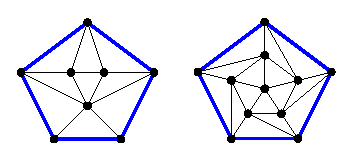
\includegraphics[width=0.9\textwidth]{images/example5.eps}
    \end{figure}
\end{frame}

\begin{frame}
    \frametitle{Example of non-reducible configurations on $R_5$.}
    \begin{figure}
        \centering
        
\includegraphics[width=0.4\textwidth]{images/example5_bad.eps}
        \caption{Replacing this configuration by our reducer yields the same graph. Therefore, this configuration does not fall under the 1-reducibility of $R_5$. If it were, then the four color theorem would proven. }
    \end{figure}
\end{frame}